\section{Block Diagram}

Figure~\ref{fig:blockDiagram} shows a revised system block diagram. It contains the model numbers of all the components, the types of connections required to the microcontroller unit (MCU) and the amount of lines needed for each connection.  An explanation of the changes made follows.

\begin{figure}[H]
\centering
	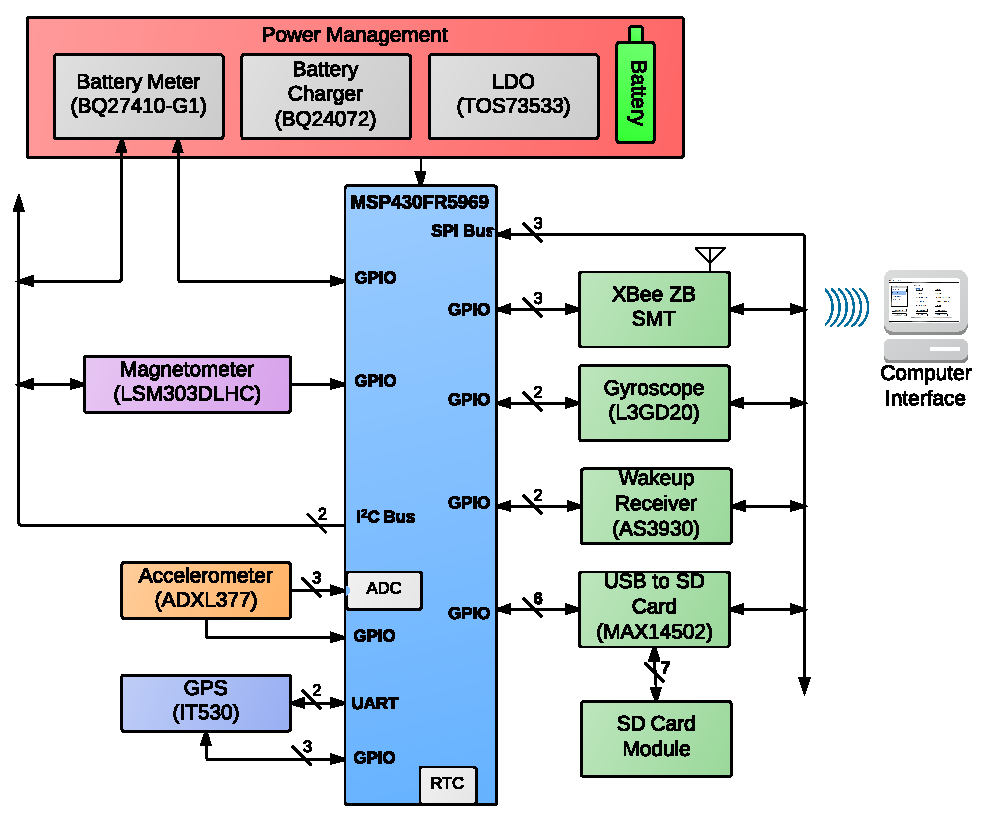
\includegraphics[width=\textwidth]{img/blockDiagram}
	\caption{System Block Diagram \label{fig:blockDiagram}}
\end{figure}

\subsection{Battery Charger and Battery Meter}

In the previous thermal analysis, it was found that the power loss in the LDO conversion was too high. This was because the LDO is fed by the battery charger and the previous battery charger had an output voltage of 5V. To avoid such power loss, the battery charger was changed.  The new battery charger's output voltage is 3.7V, so the power loss when converting to 3.3V changes significantly. This helps to stretch the battery life.  

Texas Instruments (TI) application note plans for the battery meter and battery charger to work together.  Since it was designed to work along with a different battery meter, the battery meter was changed too.

%TODO citar application note y arreglar parrafo

\subsection{Xbee and GPS}

Xbees have two modes of operation: transparent (AT) mode and API mode. API mode requires larger packets to send information, in addition to encryption and decryption functions.  This translates to the need of more RAM and program memory, more time to send data and more power consumption.  AT mode, on the other hand, is a very simple and fast to communicate between Xbees. Since this system is battery driven, it needs to have a very low power consumption.  The system also needs to transfer data between the base station and the sphere as quick as possible, because the available time to send/receive data is very short in some cases.  Also, because a lot of components are being used, memory is valuable and limited resource in this system. All these make AT mode more feasible for the application. Previously, it was stated that the communication between the Xbee and the MCU was going to be made via SPI. SPI mode requires the use of API mode, since AT mode is only available when communicating with the Xbees via UART. This is why the Xbee communication was changed from SPI to UART.

Because the chosen MCU did not have another UART port available because it is used for the GPS, two ways to make the Xbee UART communication possible were considered.  The first method considered was to add a multiplexer to the UART line to make a species of UART bus.  This implies to add another hardware component to the system.  Since the system has space limitations, this option was not very feasible.  Also, it would imply to have more power consumption.  The second method considered was to implement a software UART.  Implementing a software UART is very simple and does not requires too much program memory. Since the Xbee is going to be used more than the GPS, it is best to connect the Xbee to the hardware UART.  This will help save more power.  The GPS then will be connected to the new software UART.